\documentclass[10pt]{article}
\usepackage[utf8]{inputenc}
\usepackage[spanish]{babel}
\usepackage{amsmath}
\usepackage{epsfig}
\usepackage{enumerate}
\usepackage{float}
\usepackage{listings}
\frenchspacing
\linespread{1.2}                                          %espacio entre líneas
\setlength{\parskip}{1.5ex plus 0.2ex minus 0.2ex}        %espacio entre párrafos
\setlength{\columnsep}{0.9cm}  				  %espacio entre columnas
\usepackage{indentfirst}
\usepackage{graphicx}
\usepackage{verbatim}
\usepackage{url}
\usepackage{multicol}
\usepackage{geometry}
\usepackage{fancyhdr}
\usepackage{moreverb}
\usepackage[hidelinks]{hyperref}

\geometry{tmargin=3.0cm, lmargin=3.0cm, rmargin=2.5cm, bmargin=3.0cm}

\newcommand\R{R}
\newenvironment{keywords}{\begin{description}\item[Palabras Claves:]}{\end{description}}
%\renewcommand{\refname}{Referencias}
%\renewcommand\listfigurename{Lista de Figuras}
%\renewcommand\listoftables{Lista de Tablas}


\title{
\center{\emph{Desarrollo de una plataforma astroinformática para la administración y análisis inteligente de datos a gran escala} \\}
\center{\textbf{Identicación de Líneas Espectrales Utilizando Técnicas de Sparse Coding} \\}
\author{
        Andrés Riveros, Karim Pichara,  Diego Mardones, Paulina Troncoso, Mauricio Araya,\\
        Mauricio Solar, Marcelo Mendoza, Niel Nagar, Victor Parada, Guillermo Cabrera,\\
		Ricardo Contreras, Jorge Ibsen, Lars Nyman, Eduardo Vera, Paola Arellano,\\
		Luis Ar\'evalo, Camilo Valenzuela, Patricio Ramirez, Jos\'e Castro.	
}
\date{Santiago, \today}
}

\begin{document}
\maketitle

\vspace{0.5cm}

\begin{abstract}
	La astronomía está enfrentando nuevos desafíos en cómo analizar big data y por lo tanto, cómo buscar o predecir eventos/patrones de interés. La detección e identificación automática de líneas espectrales es un problema astronómico que aún no ha sido resuelto, por lo que actualmente la identificación se ha limitado al análisis manual de espectros por parte de radio-astrónomos. El uso de la espectroscopía permite describir la composición química de objetos astronómicos a partir de emisiones producidas por la interacción entre la radiación y la materia, originando así líneas de emisión. Nuevas observaciones en regiones de longitudes de onda antes no exploradas que estarán disponibles gracias a proyectos como el Atacama Large Millimeter Array (ALMA), con las cuales se pretende utilizar técnicas de aprendizaje de máquina para identificar automáticamente estas líneas de emisión. Con el uso de datos simulados basados en las observaciones que se han obtenido del radiotelescopio ALMA, se propone un algoritmo con el cual identificar líneas, con el fin de determinar las moléculas que componen a las galaxias observadas. Para esto se utilizará la técnica de Sparse Coding, con el cual se evaluarán las moléculas que pueden dar origen al espectro observado y se espera encontrar la mejor combinación de moléculas para recrear dicho espectro. A partir de este algoritmo, los astrónomos podrán obtener una probabilidad asociada a las posibles combinaciones de moléculas que componen los objetos astronómicos. 
\end{abstract}

\vspace{0.4cm}

\begin{keywords}
	líneas espectrales: líneas de emisión; técnica: espectroscopía; método: minería de datos.
\end{keywords}

\vspace{1cm}

\thispagestyle{empty}

\newpage

\section{Resumen Ejecutivo}

Este proyecto se desarrolla en el marco del desarrollo de un proyecto colaborativo de varias universidades chilenas para la iniciativa del Observatorio Virtual Chileno (ChiVO). ChiVO es una plataforma en línea que pondrá a disposición de los astrónomos acceso a las mediciones del radio-telescopio Atacama Large Millimeter Array (ALMA). Además, proporcionará una serie de herramientas con las cuales podrán procesar y obtener información especializada de dichas mediciones de ALMA.

El los datos que el radio-telescopio ALMA pondrá a disposición consisten en cubos de datos, en los cuales dos dimensiones son espaciales y una tercera dimensión corresponde a un rango de longitud de onda. Esto significa que se cuenta con una matriz tridimensional de la cual en cada par espacial, es posible obtener un espectrograma diferente.

La Pontificia Universidad Católica de Chile (PUC) participa con el desarrollo de una herramienta de identificación de líneas espectrales utilizando técnicas de minería de datos. Esta herramienta consiste en un algoritmo que utiliza técnicas de sparse coding para obtener la probabilidad de que distintas combinaciones de moléculas que den origen a los espectrogramas observados.

Dado que en la fase en la que se encuentra el proyecto no se cuenta con datos reales, se utilizarán datos simulados con las características de las futuras mediciones de ALMA. Para esto se utilizará el software de simulación ASYDO, desarrollado en conjunto con este proyecto como parte de las herramientas disponibles en el proyecto ChiVO.

Con este conjunto simulado de espectros, se pretende identificar líneas espectrales a partir de un conjunto de moléculas con las cuales fueron simuladas dichos espectros. Se espera poder recuperar este conjunto de moléculas solo con el espectrograma observado. El resultado será una distribución de pertenencia de estas líneas espectroscópicas a diferentes configuraciones de moléculas.

La particularidad del algoritmo de identificación propuesto radica en la incorporación del factor probabilista en la identificación de los espectros, al consistir el resultado del algoritmo en una probabilidad en vez de un resultado determinista. Además, la automatización de este proceso permitirá entregar a los astrónomos una herramienta con la cual obtener una primera aproximación a la solución de este problema.

A lo largo del documento se detalla el estado del arte del problema, la metodología con la cual se espera resolver el problema, el enfoque con el que será abordado el problema, la especificación de requerimientos del algoritmo a desarrollar, se describirá el prototipo de la solución propuesta, con su diseño e implementación y la validación final.

\newpage

\tableofcontents
\newpage

\listoffigures
\newpage

\listoftables
\newpage

\section{Metodología de Trabajo}

En la metodología de trabajo se detalla el proceso a través del cual el problema a solucionar fue concebido, los obstáculos que ha presentado y los pasos seguidos para hallar la solución al problema.

Este proyecto surge de la potencial capacidad de la minería de datos de ser utilizados como herramienta para la astronomía. La dificultad de los problemas astronómicos complejos utilizando minería de datos radica en que estos involucren una gran cantidad de datos a ser procesados.

ChiVO pondrá a disposición herramientas que utilizarán datos de ALMA, por lo que la cantidad de datos de mediciones astronómicas a procesar crecerá exponencialmente. Es por esto que una herramienta que automatice el procesamiento de dichos datos y entregue información útil y especializada a astrónomos será de gran utilidad.

La metodología se puede separar en varias etapas para resolver el problema en cuestión:


\begin{description}
\item [Definición del problema] Identificación de problemas a resolver: Se debe acotar el problema, definir el tipo de datos que se utilizarán, en este caso la simulación de datos tipo ALMA. Esto último lleva a la siguiente etapa:

\item [Simulación de datos] Especificaciones: Se deben definir con los parámetros de la simulación, así como un subconjunto de moléculas, en conjunto con astrónomos. Para esto deben considerarse las limitaciones de la simulación.

\item [Estado del arte] Se estudiará el estado del arte en la clasificación de líneas espectrales. Se buscarán situaciones similares con el fin de aplicar técnicas adecuadas a este caso. Finalmente, para la codificación de espectros en variables que representen las moléculas presentes, se buscará una representación en base a trabajos previos en el área, como las aplicaciones para la determinación de compuestos existentes en espectros de Ranman \cite{howley_effect_2005}.

\item [Desarrollo de la solución] se realizará una iteración de soluciones al problema de codificación sparse, analizando el efecto de los parámetros en los modelos a utilizar y determinando la cantidad de parámetros necesarios para abarcar mayor complejidad en la identificación de los espectros.
\end{description}



\newpage

\section{Definición del Problema}

En una etapa inicial, se efectuaron una serie de reuniones administrativas con el conjunto de universidades que colaboran en el proyecto ChiVO. En estas reuniones se buscaba establecer como abordar y en qué se centraría cada universidad. El objetivo era desarrollar herramientas para los astrónomos que fueran útiles e innovadoras, y que utilizaran los datos que estarán disponibles a partir de ALMA.

Así surgió la idea de desarrollar herramientas que aplicaran técnicas de minería de datos. Con los astrónomos involucrados en el proyecto fue posible realizar una propuesta de un problema astronómico. Cada proyecto de las universidades involucradas resolvería dicho problema con un enfoque diferente.

La información que el radio-telescopio ALMA entregará consiste en cubos de datos con dos dimensiones espaciales y una dimensión de longitud de onda. En cada par espacial se mide el brillo de temperatura para un rango de longitudes de onda, o su equivalente en una frecuencia determinada.

\begin{figure}[H]
	\begin{center}
		
\includegraphics[width=140mm]{images/fig1}
		\caption{Cubo de datos de ALMA, con dos dimensiones espaciales y una dimensión de frecuencia.}
	\end{center}
\end{figure}

Producto de la radiación que emiten los objetos estelares, y de su interacción con la materia, se generan líneas de emisión. Esta líneas de emisión son caracteríaticas para ciertos niveles de energía de las moléculas que conforman los objetos astronómicos. La detección de las líneas de emisión y posterior asociación con las moléculas que las originan, permite conocer la composición de los objetos estelares.

La combinación de estas líneas de emisión para cada objeto permite obtener una huella digital de este, única, dadas sus características internas y diferentes factores como la temperatura del objeto, la velocidad con la que viaja por el espacio, etc.

Con esta información, se contaría con una gran cantidad de líneas espectrales, por lo que surge la idea de detectar dichas líneas espectrales como un problema astronómico de interés para aplicar técnicas de minería de datos.

Por el lado de la minería de datos, se contará con suficientes datos para técnicas y desarrollar un algoritmo de identificación automática. Por parte de los astrónomos, se podrá contar con una herramienta que automatice la identificación de líneas de emisión en espectrogramas pertenecientes a objetos astronómicos.

Cabe destacar que el objetivo del algoritmo es que apoye la rigurosidad de una clasificación hecha por un experto, al servir como preprocesamiento inicial para que este clasifique sus líneas, por lo que no busca reemplazar totalmente la labor del experto, y se espera un márgen de error para ciertos casos identificables.

Luego de definir el problema, era necesario determinar un set de datos con el cual comenzar a desarrollar el algoritmo. Dada la cantidad necesaria de espectros para desarrollar un modelo predictivo, y como actualmente no se cuenta con mediciones suficientes del radio-telescopio, se optó por utilizar una simulación de espectros.
\newpage

\section{Simulación de Datos}

Para el desarrollo del algoritmo de identificación de líneas espectrales se utilizará el servicio web de datos simulados que proporcionará ChiVO. Este proyecto, llamado Astronomical SYntetic Data Observatory (ASYDO) se desarrolla en paralelo a este proyecto como parte de las herramientas que podrán utilizar los astrónomos como servicio web. Dicho proyecto está disponible en \footnote\url{https://github.com/ChileanVirtualObservatory/ASYDO}.


La simulación permitirá generar un set de entrenamiento para desarrollar el algoritmo de identificación propuesto en este proyecto. Al ser este servicio de simulación un input importante para el desarrollo del algoritmo, se han realizado una serie de reuniones para trabajar conjuntamente y obtener un set de datos simulados adecuado.

Con la ayuda de los astrónomos que participan en el proyecto ChiVO se ha determinado los parámetros necesarios para llevar a cabo la simulación. Se ha definido la complejidad y la importancia de replicar características determinadas que ayudarán a obtener curvas de espectros que se acerquen lo suficiente a los datos que se espera obtener a partir de las observaciones de ALMA.

Para que el algoritmo sea correctamente desarrollado con datos simulados, se deberá incluir en la meta-data de los cubos las líneas de emisión presentes en los espectros. Con esto será posible evaluar el modelo predictivo y determinar métricas para validar las predicciones.

Las características de las mediciones de ALMA han permitido obtener las siguientes especificaciones a la hora de simular cubos de datos tipo ALMA:

\begin {table}[H]
\begin{center}
	\begin{tabular}{|c|c|}
		\hline Ancho de banda espectral & 4000 MHz \\ 
		\hline Resolusión espectral & 1 MHz \\ 
		\hline 
	\end{tabular}
	\caption {Especificaciones comúnes para todos los cubos de datos simulados}
\end{center}
\end{table}

Y como parámetros de entrada, el usuario tendrá que proporcionar:

\begin {table}[H]
\begin{center}
	\begin{tabular}{|c|c|}
		\hline Frecuencia central &  MHz \\ 
		\hline Resolusión espectral & 1 MHz \\ 
		\hline Asención &  Grados \\ 
		\hline Declinación & Grados \\ 
		\hline Ancho de las lineas & (fwhm) \\ 
		\hline 
	\end{tabular}
	\caption {Parámetros proporcionados por el usuario para los cubos de datos simulados}
\end{center}
\end{table}

Con el fin de representar las mediciones de manera cercana a la realidad, se escogió con la ayuda de los astrónomos un set de moléculas y sus respectivos isótopos. El criterio consistió en seleccionar moléculas con una estructura que no fuera en exceso complicada, de forma que no supusieran una complejidad innecesaria para el algoritmo. Además, este set de moléculas debía ser representativo de las moleculas que se esperan encontrar en los objetos astronómicos. Estas se muestran en la siguiente tabla.

\begin {table}[H]
\begin{center}
	\begin{tabular}{|c|c|c|}
		\hline Nombre & Fórmula &  Isótopos \\ 

		\hline 	Carbon Monoxide & 'CO' & 'COv=0','COv=1','13COv=0','C18O'\\
								&	   & 'C17O','13C17O','13C18O' \\
		
		\hline	Diazenylium & 'N2H' & 'N2H+v=0', 'N2D+', '15NNH+', 'N15NH+' \\
			
		\hline	Cyanide Radical & 'CN' & 'CNv=0', '13CN', 'C15N' \\
			
		\hline	Hydrogen Cyanide & 'HCN' & 'HCNv=0', 'HCNv2=1', 'HCNv2=2','HCNv3=1' \\
								 &       & 'HC15Nv=0', 'H13CNv2=1', 'H13CNv=0'\\ &       & 'HCNv1=1', 'HCNv3=1', 'DCNv=0'\\ &       & 'DCNv2=1', 'HCNv2=4',  'HCNv2=1 1-v2=4 0' \\
						
		\hline  Carbon Monosulfide & 'CS' & 'CSv=0', '13C34Sv=0', 'C36Sv=0'\\
						    	   &      & 'C34Sv=0', 'CSv=1-0', '13CSv=0'\\
							       &      & 'C33Sv=0', 'CSv=1', 'C34Sv=1' \\
			
		\hline	Thioxoethenylidene & 'CCS' & 'CCS', 'C13CS', '13CCS', 'CC34S' \\
			
		\hline	Hydrogen sulfide & 'H2S' & 'H2S', 'H2S', 'H234S', 'D2S' \\
			
		\hline	Thioformaldehyde & 'H2CS' & 'H2CS', 'H213CS', 'H2C34S' \\
			
		\hline	Sulfur Dioxide & 'SO2' & 'SO2v=0', '33SO2', '34SO2v=0', 'SO2v2=1' \\
			
		\hline	Sulfur Dioxide & 'OSO' & 'OS18O', 'OS17O' \\
			
		\hline	Formaldehyde & 'H2CO'  & 'H2CO', 'H2C18O', 'H213CO' \\
			
		\hline	Formylium & 'HCO'  & 'HCO+v=0', 'HC18O+', 'HC17O+', 'H13CO+' \\
			
			
		\hline	Cyanobutadiyne & 'HC5N' & 'HC5Nv=0', 'HC5Nv11=1', 'HCC13CCCN'\\
							   &        & 'HCCCC13CN', 'HCCC13CCN', 'H13CCCCCN'\\
							   &        & 'HC13CCCCN' \\
			
		\hline	Methanol & 'CH3OH' & 'CH3OHvt=0', '13CH3OHvt=0 ', 'CH318OH' \\
						 &      & 'CH3OHvt=1 ', '13CH3OHvt=1'\\

		\hline 
	\end{tabular}
	\caption {Conjunto de moléculas e isótropos con los que se realizaron las simulaciones.}
\end{center}
\end{table}

\newpage

\section{Estado del Arte}
La determinación de líneas espectrales según el método tradicional se limitaba al análisis manual de datos para encontrar parámetros moleculares que permitan asociar los peaks en las mediciones de los espectrogramas a moléculas en ciertos estados de energía.

La falta de escalabilidad de técnicas que no automatizadas, y lo poco práctico que resultan dichos método para grandes cantidades de datos \cite{Schilke2001}, añadido a la dificultad a la hora de predecir nuevas coincidencias entre frecuencias y moléculas dada por las superposiciones de líneas, ha impulsado a los astrónomos a buscar la automatización de esta tarea.

El problema de mezclas de líneas y superposiciones son producto de tanto ruido como la falta de sensibilidad  para distinguir entre dos líneas en frecuencias cercanas. Lo anterior también puede producir peaks dobles en ciertas líneas \cite{Cernicharo2013}.

Un problema importante a la hora de identificar frecuencias subyace en líneas ópticamente delgadas, que tienden a dar resultados incorrectos. Usualmente, el uso de líneas de isotopos para su corrección resulta en un proceso costoso en tiempo y por lo mismo no es apto para datos masivos \cite{Schilke2001}.

Nummelin et al. \cite{Nummelin1998} propone el uso de un ajuste manual de las líneas a una forma arbitraria dada por una gausiana, obteniendo por cada línea su frecuencia observada, el peak en el brillo de temperatura y el ancho de la velocidad (ancho total a media altura), para así proceder con la identificación de la línea al asociarla con una molécula en cierto estado de energía. 

Para la identificación de líneas considerando las relaciones entre brillo de temperatura en un mismo espectro, es necesario asumir temperatura y origen homogéneo, dado que la diferencia de temperatura cambia la relación en serie de intensidades de líneas hiper-finas \cite{Nummelin2000}. 

Esto es importante a la hora de utilizar datos simulados con el fin de representar fielmente las características físicas de las estructuras a utilizar para entrenar, de modo que el modelo sea posteriormente aplicable sin mayores variaciones al utilizar datos reales de ALMA.

Es posible detectar patrones en las líneas que corresponden a la misma molécula e ispotropo a partir de intensidad relativa considerando que existe una razón entre diferencias de velocidad que es constante para un conjunto de líneas de emisión. Esto permite buscar patrones no tan solo de manera individual, sino que a través del análisis manual de series de líneas que se asocian a una misma molécula o átomo en sus diferentes estados energéticos. 

Los esfuerzos para desarrollar una herramienta automática de detección de líneas actualmente apuntan a herramientas semi-automáticas que utilizan como base complejos modelos físicos y químicos para la clasificación de líneas. 

XCLASS \footnote{\url{https://www.astro.uni-koeln.de/projects/schilke/XCLASS}}, 
CASSIS \footnote{\url{http://cassis.cesr.fr}} y 
WEEDS \footnote{\url{https://www.iram.fr/IRAMFR/GILDAS}} 
son herramientas que apuntan a modelar la composición de los espectros de tal forma que las simulaciones se asemejen a lo observado, existiendo grandes esfuerzos en realizar dichos modelamientos para solo la identificación de líneas. \cite{Schilke2011}.

Estas herramientas hacen uso de catálogos que contienen información sobre líneas espectroscópicas de moléculas y sus frecuencias teóricas de laboratorio, las que están disponibles públicamente en catálogos como (JPL \footnote{\url{http://spec.jpl.nasa.gov}}, 
CDMS \footnote{\url{http://www.astro.uni-koeln.de/cdms}}, 
Toyama \footnote{\url{http://www.sci.u-toyama.ac.jp/phys/4ken/atla}}) 
\cite{Schilke2011}, los que han sido compilados en 
Splatalogue \footnote{\url{http://www.splatalogue.net}} 
\cite{Remijan2008, Remijan2010}.

Las técnicas anteriormente descritas no son escalables al no ser procesos automatizados y depender de análisis o ajustes manuales que con la inminente llegada de enormes cantidades de datos provenientes de instrumentos como ALMA, dejan de ser aplicables. Por esto es necesario buscar algoritmos de clasificación que deleguen la tarea de identificar y clasificar líneas espectrales.
\newpage

\section{Desarrollo de la solución}

\subsection{Solución Propuesta}

El algoritmo propuesto tiene como propósito la identificación de los componentes moleculares que forman parte de diferentes objetos astronómicos a simular. Para esto, se analizan las líneas  espectrales a partir de los espectros de dichos objetos astronómicos, con el fin de encontrar patrones y predecir su composición.

Para un objeto astronómico, observar sus líneas espectrales puede ayudar a identificar las moleculas que lo componen, dado que para cada estado energético de dichas moléculas, al estar estas presentes en el objeto, se manifiestan en líneas de emisión a lo largo de sus espectros observados en determinadas frecuencias.

El algoritmo toma ventaja de este comportamiento y busca patrones según la presencia de ciertas líneas. Cuando una molecula está presente en la composición de un objeto, probablemente deberían observarse una serie de líneas a lo largo del espectro. Esto significa quee a menor cantidad líneas teóricas observadas de dicha molécula, menor será la probabilidad de que la molécula forme parte de la composición del objeto.

Así, si existe confusión a la hora de identificar una línea espectroscópica entre dos moléculas, es posible realizar una predicción probabilista de la molécula a la cual corresponde dicha línea basándose en la presencia de cada línea teórica a lo largo del espectro que se está observando.


\subsection{Diseño del Prototipo}

Como se mencionó anteriormente, para el diseño del prototipo se utilizó el proyecto ASYDO. La temperatura en estas simulaciones no posee unidades, ya que las magnitudes de las líneas son relativas a la línea más alta de CO, a la cual se le ha asignado un valor arbitrariamente. Esto significa que los valores en sí mismos no poseen un significado.

El proceso para simular los cubos de prueba consistió en encontrar todas las moléculas y todos sus isotopos dentro de un rango de frecuencia. El rango de frecuencia utilizado para estas pruebas fue desde los 602000 MHz hasta los 606000 GHz, aproximadamente, que corresponde a la banda 9 de ALMA. Se corrió un script de líneas combinadas de varios subconjuntos aleatorios de isotopos, subconjunto de tamaño variable del total de moléculas teóricamente existentes en esta ventana de frecuencias utilizada.

El objetivo del algoritmo es entonces recuperar la lista de moléculas con la cual se generaron los cubos de datos. Para realizar esta tarea solo se pueden utilizar los espectrogramas observados. A través de métodos estadísticos se pretende predecir la presencia de ciertas moléculas y validar dichas predicciones al conocerse las moléculas utilizadas para generar las simulaciones.


\begin{figure}[H]
	\begin{center}
		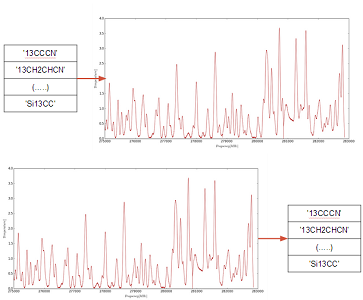
\includegraphics{images/fig0}
		\caption{Se desea recuperar la lista de moléculas con la que se simuló el espectrograma. }
	\end{center}
\end{figure}



\subsection{Implementación}

El código de la implementación se encuentra disponible en el repositorio del proyecto de ChiVO en git. \footnote{\url{https://github.com/ChileanVirtualObservatory/DISPLAY}}

\subsubsection{Etapa de Detección}

El proceso de detección de líneas utiliza un parámetro de sensibilidad que determina si una medición es considerada una potencial línea espectroscópica. Esta sensibilidad depende de la desviación estándar del ruido en una región sin líneas visibles. Para obtener este parámetro se forzó a que en cada cubo, el pixel (0 , 0) no tuviese líneas espectrales, sino que solo ruido. Esto en la práctica se puede obtener seleccionando una región vacía del cubo de datos que el usuario previamente seleccione.

\begin{figure}[H]
	\begin{center}
		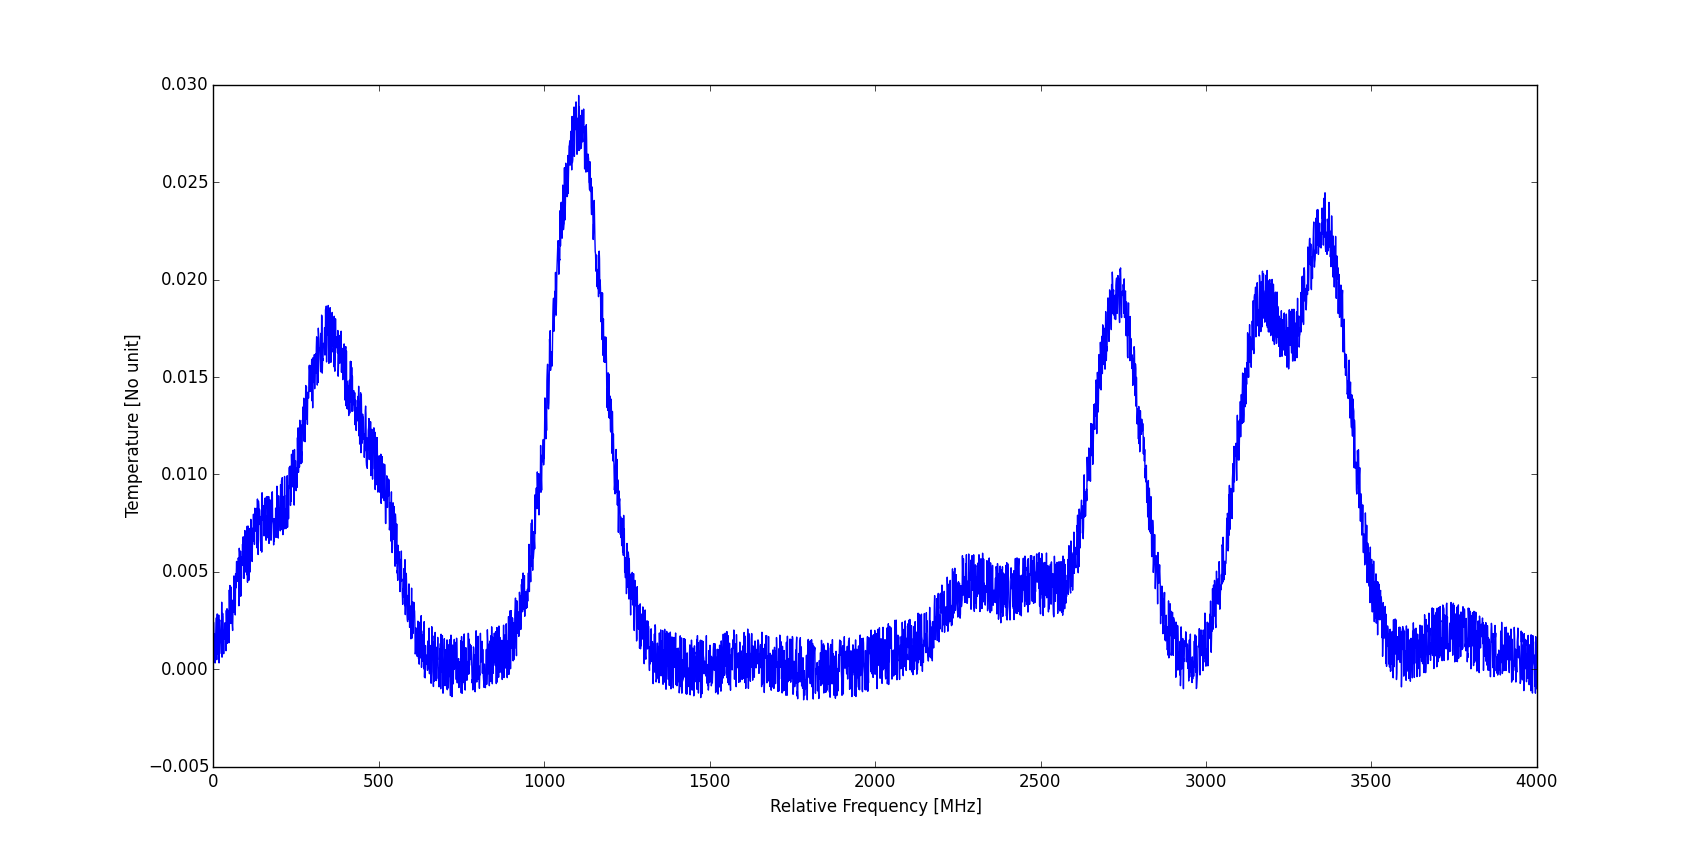
\includegraphics[width=140mm]{images/fig2}
		\caption{Espectro al situarse en un píxel espacial en particular. }
	\end{center}
\end{figure}

A continuación, para cada punto espacial del cubo de datos, se toma cada espectrograma de manera independiente. Lo primero es reducir el ruido de el espectro utilizando un filtro de Savitzky-Golay \cite{howley_effect_2005}. Este filtro utiliza un parámetro que indica el número de mediciones consecutivas a utilizar para suavizar la curva, por lo que el ancho de las curvas simuladas corresponde aun buen parámetro para ser asignado. Con este filtro se puede obtener un espectro con menor variación y así, identificar con mayor claridad las líneas. Este filtro se aplica al cubo completo, incluido el píxel con solo ruido, para hacer comparables los espectros al calcular la sensibilidad.

\begin{figure}[H]
	\begin{center}
		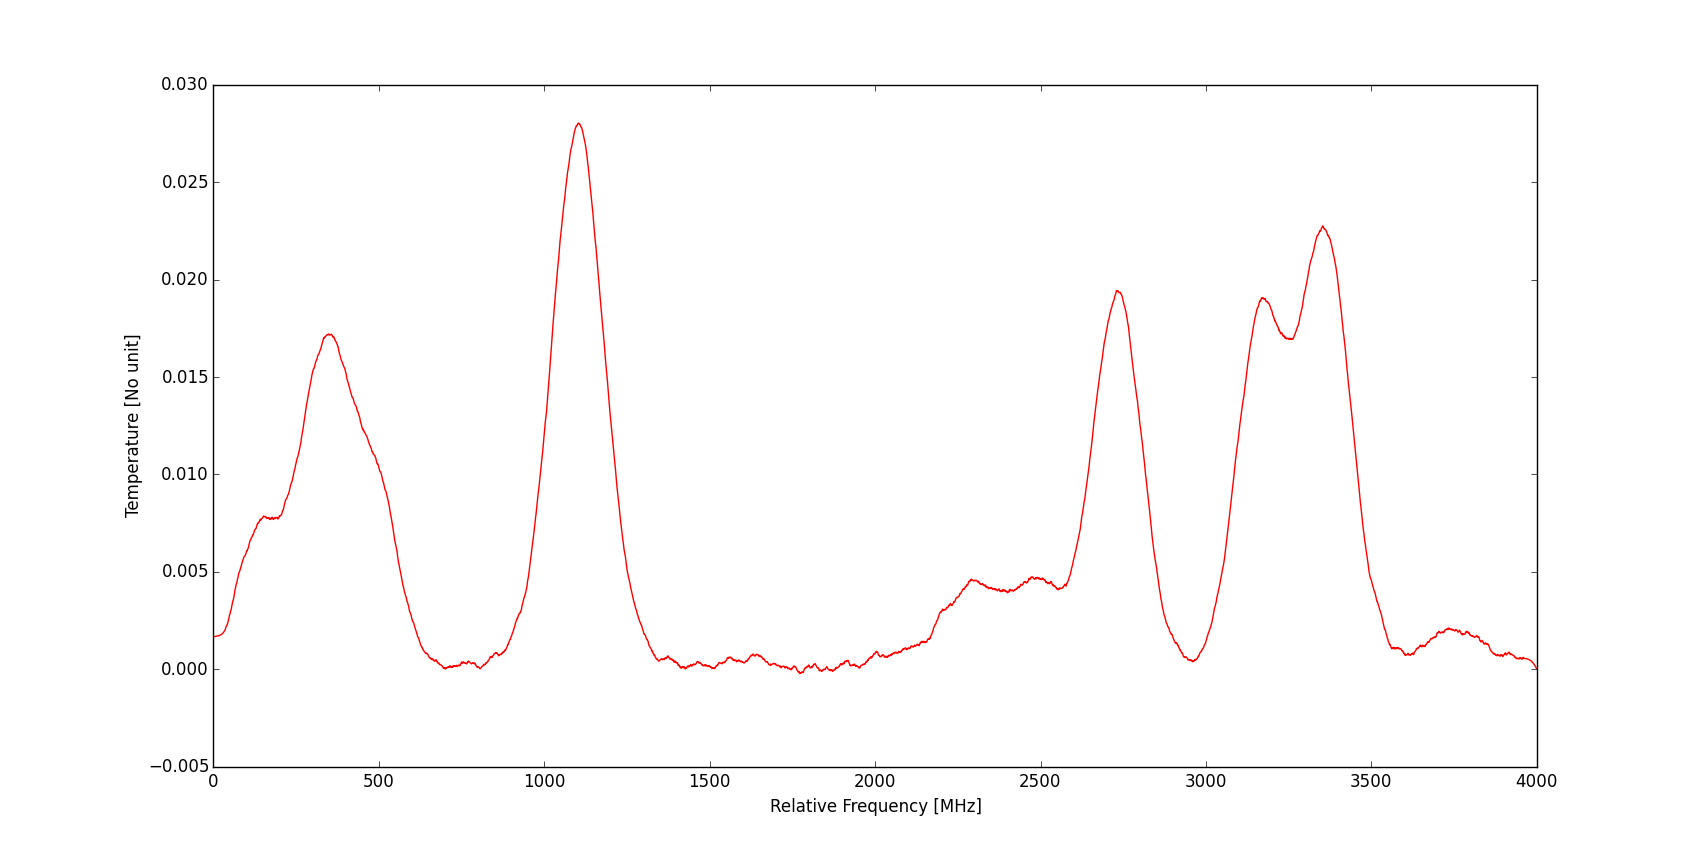
\includegraphics[width=140mm]{images/fig3}
		\caption{Espectro al reducir el ruido con un filtro de Savitzky-Golay. }
	\end{center}
\end{figure}


Se comienza con la determinación de los puntos máximos de la curva observada. Es posible asignar un parámetro que determina la distancia máxima que debe existir entre el brillo de dos frecuencias consecutivas para ser considerados un máximo. Sin este parámetro, la curva tendría una serie de falsos máximos y mínimos producto del ruido existente en las mediciones. Así, cada máximo local detectado que está por sobre el parámetro de sensibilidad es un candidato a línea de emisión.

\begin{figure}[H]
	\begin{center}
		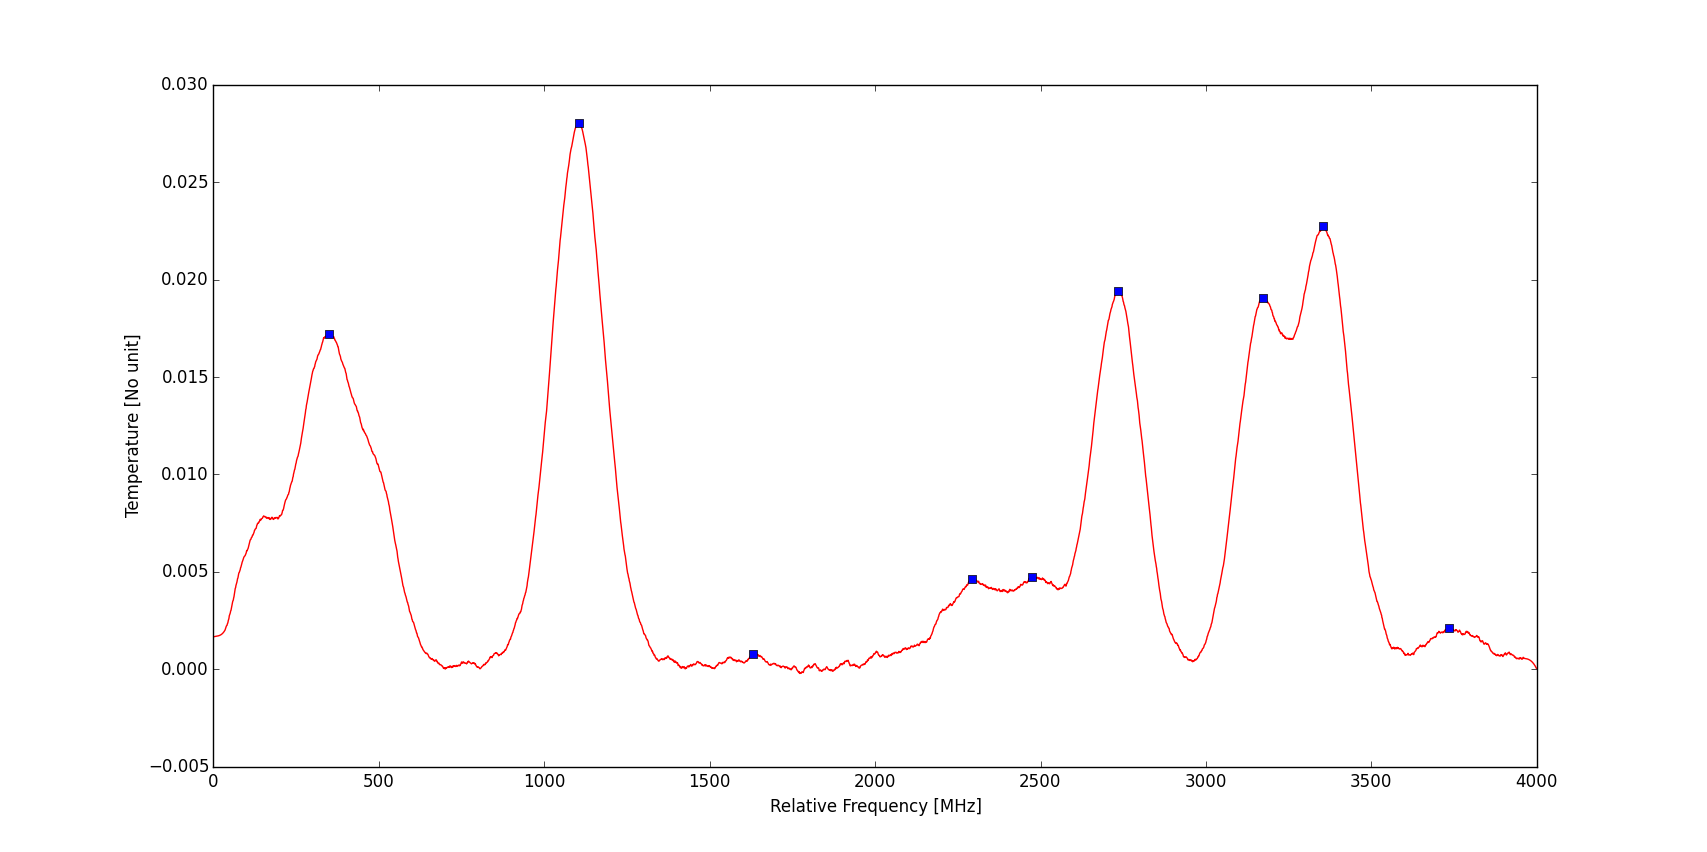
\includegraphics[width=140mm]{images/fig4}
		\caption{Puntos máximos locales por sobre el parámetro de sensibilidad. }
	\end{center}
\end{figure}

Al final del proceso, se crea un vector del tamaño del ancho de banda observado, donde se cada elemento del vector representa 1 Mhz del espectro. En cada frecuencia donde se detectó una línea, se asigna el valor 1, y cero en caso contrario.

\begin{figure}[H]
	\begin{center}
		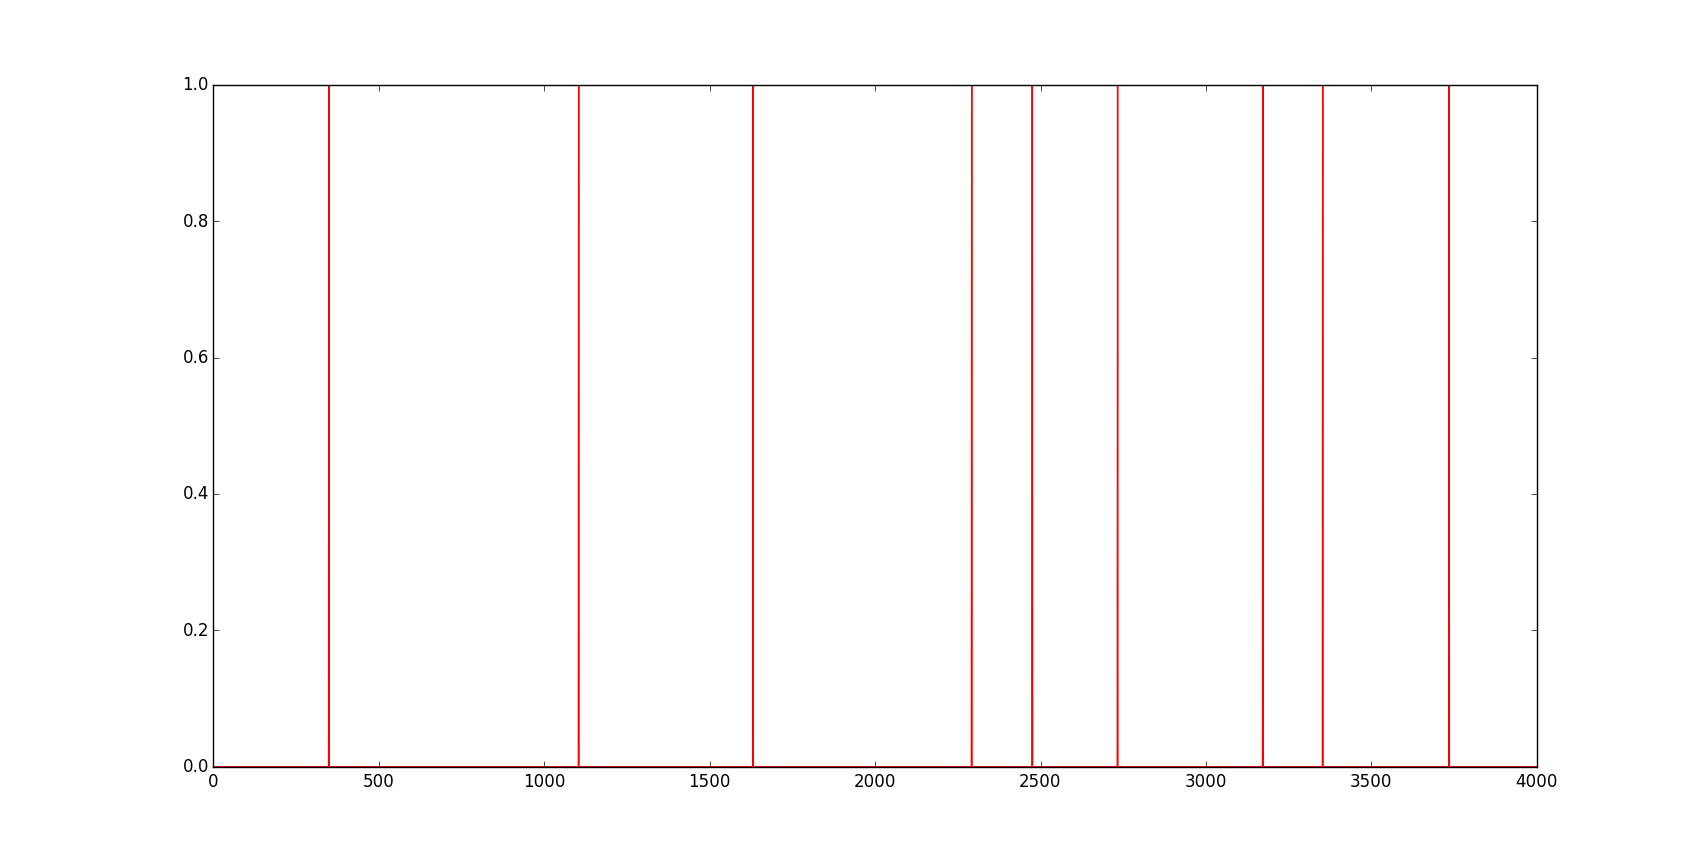
\includegraphics[width=140mm]{images/fig5}
		\caption{Gráfico del vector observado con valores no nulos en los puntos detectados. }
	\end{center}
\end{figure}

\begin {table}[H]
\begin{center}
	\begin{tabular}{|c|c|c|c|c|c|c|c|c|c|c|}
		\hline 0 & 0 &  ... &  1 & ... &  1 & ... & 1 & ... & 0 & 0 \\ 
		\hline
	\end{tabular}
	\caption {Forma del vector del espectro observado para el caso analizado.}
\end{center}
\end{table}

\subsubsection{Etapa de Predicción}

A continuación, se utiliza el catalogo de líneas espectroscópicas teóricas Splatalogue para obtener la lista de todas las frecuencias teóricas en el rango observado.

Para cada isotopo con líneas teóricas, se crea un vector del tamaño de la ventana en Mhz, similar al de la etapa de detección, donde el valor de cada posición es 1 si existe una línea teórica en dicha frecuencia para dicho isotopo, y cero en otro caso. Cada uno de estos vectores corresponde a una palabra de un diccionario de moléculas.

Posteriormente, se procesan las palabras de modo que solo tengan valores distintos de cero en las frecuencias donde el espectro observado es distinto de cero. Para esto, se asigna en dichas frecuencias la diferencia entre 1 y distancia exponencial entre la frecuencia observada y la frecuencia teórica más cercana, utilizando como parámetro sigma igual al ancho de las líneas espectrales.

Con esto se espera que las palabras que tienen frecuencias teóricas más cercanas a las observadas, tendrán valores mayores, con lo que el algoritmo de sparse coding tenga preferencia a elegir dichas palabras.

\begin{figure*}[ht]
	\centering
	\subfigure[Figura 6.1.]{
		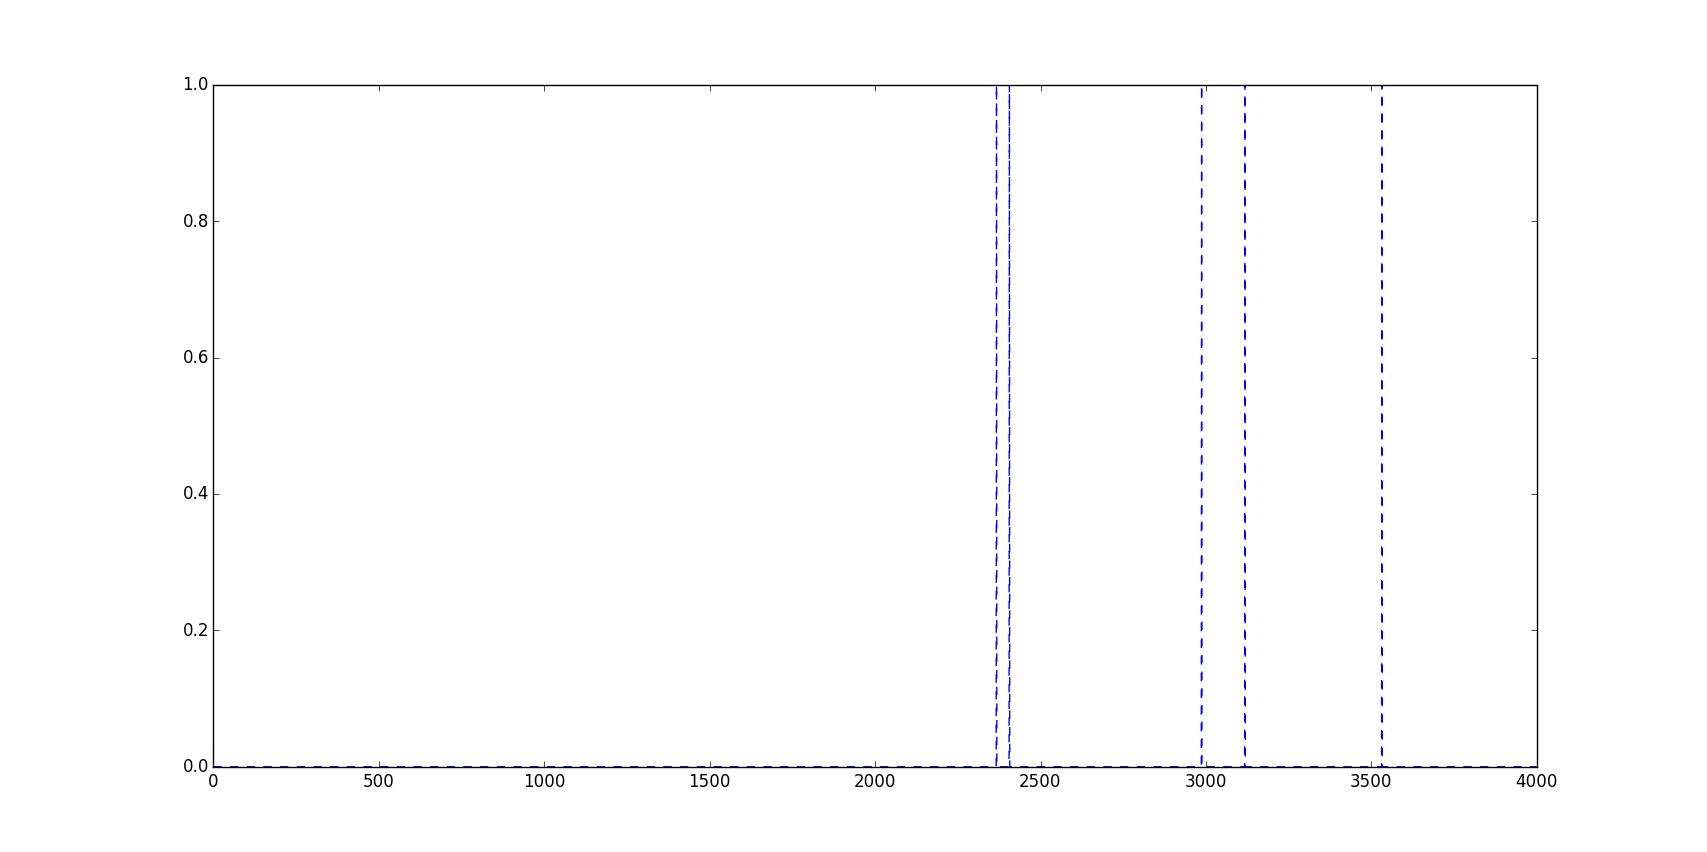
\includegraphics[width=100mm]{images/fig6-1}
	\label{fig6-1}
	}
	\subfigure[Figura 6.2.]{
		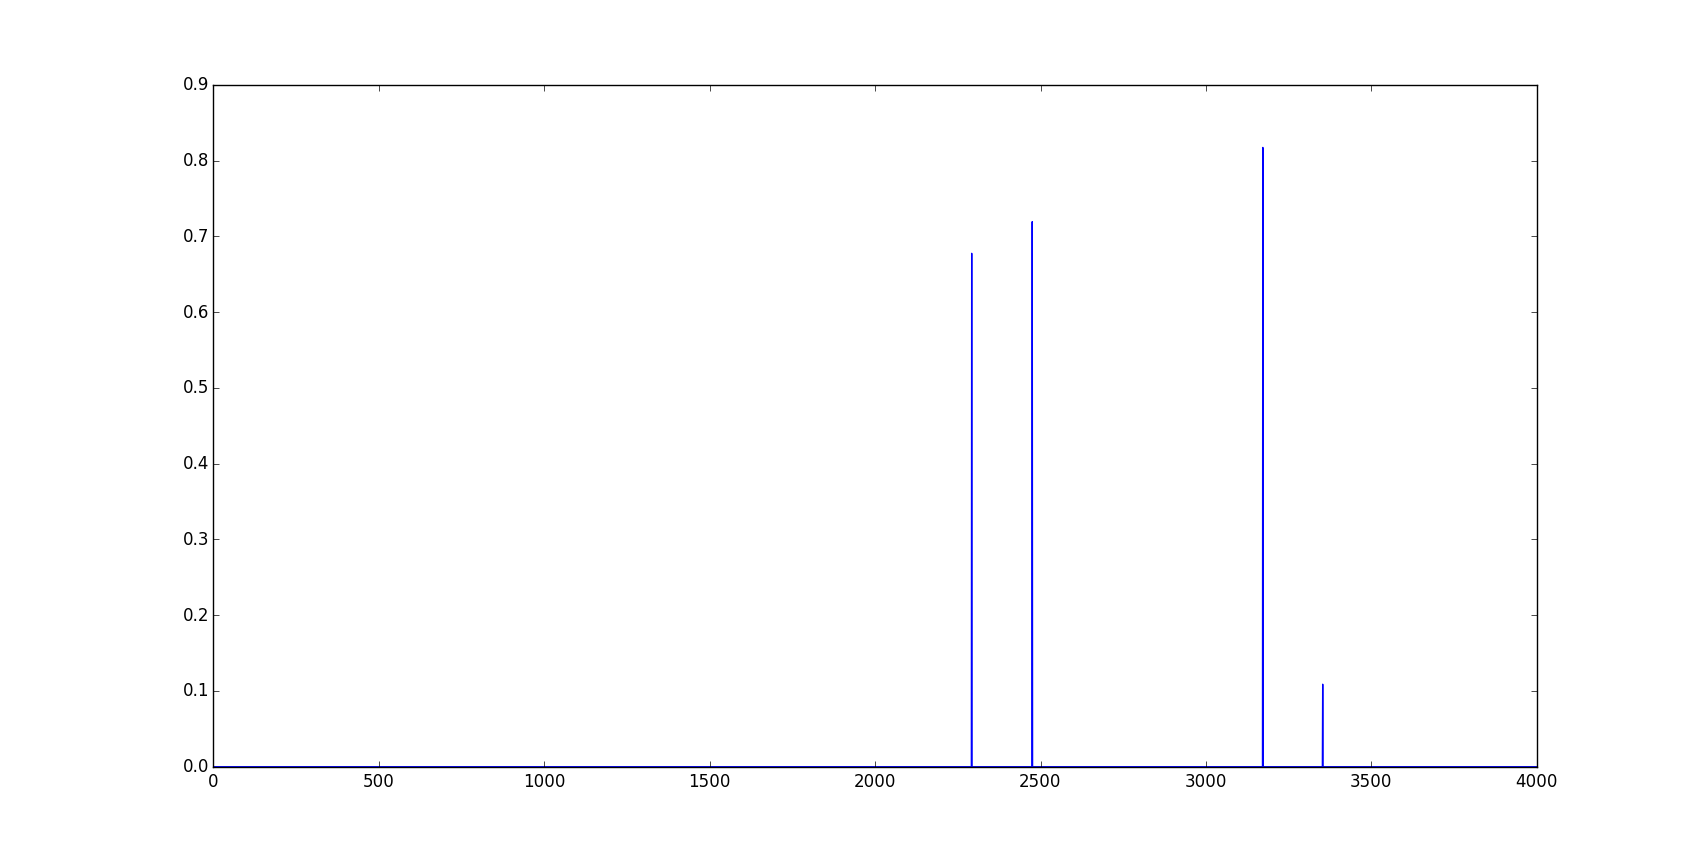
\includegraphics[width=100mm]{images/fig6-2}
		\label{[fig6-2]}
	}
	\caption{Rn la figura \ref{subfig:fig6-1} se grafica una palabra teórica y en la \ref{fig6-2} su equivalente recalculado}
\end{figure*}

La implementación se asegura de que cada frecuencia teórica cambie el valor de una y solo una frecuencia observada, y en caso de que haya otra frecuencia teórica que también tenga como frecuencia observada más cercana a la misma frecuencia, se asigna la menor distancia a dicha frecuencia observada. Con esto, cada palabra del diccionario queda con la misma o con menor cantidad de frecuencias distintas de cero.

\begin {table}[H]
\begin{center}
	\begin{tabular}{|c|c|c|c|c|c|c|c|c|c|c|c|}
		\hline Vector Obervado     & 0 & 0 &  0 &  1    & 0 &  1 & 0 & 1   & 0 & 0 & 0 \\ 
		\hline Palabra Teórica     & 0 & 0 &  1 &  0    & 0 &  1 & 0 & 0   & 0 & 0 & 1 \\ 
		\hline Palabra Recalculada & 0 & 0 &  0 &  0.88 & 0 &  1 & 0 & 0.6 & 0 & 0 & 0 \\ 
		\hline
	\end{tabular}
	\caption {Ejemplo de recálculo de una palabra utilizando para la distancia exponencial sigma = 2.}
\end{center}
\end{table}

Finalmente, se tiene un problema de optimización con una formulación de sparse coding, donde se intenta acercar  al máximo la combinación lineal entre palabras de tal forma que se construya el vector del espectro observado. El paramero de sparsity permite restringir la cantidad de palabras que se desea que el modelo utilice para formar la observación. En este caso se asignó un valor elevado para que el modelo pudiese acercarse lo máximo posible a la observación sin límite de palabras.  La función a minimizar en esta formulación es la norma l-2 y corresponde al error cuadrático medio.


\begin{center}
$min_{\alpha} ||x-D\alpha||_2^2$ 
$s.a.$ 
$||\alpha||_1 \leq \lambda$ \\
$x$ : vector observado, 
$D$ : diccionario recalculado, 
$\lambda$ : parámetro de spartity, 
$||()||_2$ : Norma l-2
\end{center}


La solución óptima debería utilizar solo las palabras asociadas a los isotopos presentes en el espectro. En la siguiente tabla se puede ver la simulación realizada y los isotopos rescatados:

\begin {table}[H]
\begin{center}
	\begin{tabular}{|c|c|c|}
		\hline Nombre & Fórmula &  Isótopos \\ 
		

		\hline	Hydrogen Cyanide & 'HCN' & 'HC15Nv=0', 'H13CNv2=1', 'H13CNv=0'\\ 
		
		\hline	Thioformaldehyde & 'H2CS' & 'H213CS' \\
		
		\hline	Sulfur Dioxide & 'SO2' & 'SO2v=0', 'SO2v2=1' \\
		
		\hline	Sulfur Dioxide & 'OSO' & 'OS18O', 'OS17O' \\
		
		\hline	Formaldehyde & 'H2CO'  & 'H2C18O', 'H213CO' \\
				
		\hline 
	\end{tabular}
	\caption {Conjunto de isótropos con los que se realizaron simuló la implementación.}
\end{center}
\end{table}

\begin {table}[H]
\begin{center}
	\begin{tabular}{|c|c|c|c|}
		\hline Nombre & Fórmula &  Isótopos & Alpha \\ 
		
		
		\hline	Hydrogen Cyanide & 'HCN'  & 'HC15Nv=0' & 0.0000\\
								 &		  & 'H13CNv2=1' & 0.0000\\
								 &		  & 'H13CNv=0' & 0.0000\\ 
								
		
		\hline	Thioformaldehyde & 'H2CS' & 'H213CS' & 0.0000\\
		
		\hline	Sulfur Dioxide & 'SO2'	  & 'SO2v=0' & 0.0000\\
								&		  & 'SO2v2=1'& 0.2694 \\
		
		\hline	Sulfur Dioxide & 'OSO' & 'OS18O' & 0.9612\\
							   &	   & 'OS17O' & 0.5589\\
		
		\hline	Formaldehyde & 'H2CO'  & 'H2C18O' & 0.0000\\
							 &		   & 'H213CO' & 0.0000\\
		
		\hline 
	\end{tabular}
	\caption {Conjunto de isótropos utilizados para la simulación y su valor de alpha.}
\end{center}
\end{table}

Cabe destacar que en este caso solo hubo un falso positivo, el isotopo '33SO2', con un valor de alpha de 0.6592. Esto significa que el algoritmo tiende a elegir los isotopos de moléculas con mayor cantidad de líneas en el ancho de banda observado, y es un aspecto a mejorar. 

Además, ciertas moléculas no son detectadas, y esto se puede deber a dos factores: en primer lugar, el algoritmo no logró detectarlas en la etapa anterior al no ser suficiente el filtro de ruido aplicado para que fuera identificada como máximo local o, en segundo lugar, no superó la sensibilidad dado que la variabilidad de la simulación hizo que no fuera observable. 

%\begin{figure}[H]
%	\begin{center}
%		
\includegraphics{images/fig1}
%		\caption{Espectro residual al sustraer una gausiana ajustada en una potencial línea de emisión. }
%	\end{center}
%\end{figure}

% Una forma de validación del algoritmo consiste en tomar un solo punto espacial del cubo como entrenamiento del algoritmo, y el resto de los pixeles como test de validación. De esta forma las palabras teóricas se recalcularán según las observaciones de dicho píxel espacial. En el resto de los píxeles del cubo, la variabilidad producto del effecto doppler interno y propia de la simulación  debería generar variaciones de forma que ciertas líneas se manifestarían y ciertas dejarían de observarse, a pesar de tener la misma composición.

% Si el algoritmo puede predecir los compuestos detectados en el píxel de referencia en el resto del cubo, se validaría esta aproximación al problema. De esta forma, se procedió a evaluar el algoritmo, obteniendo los siguientes resultados:




\newpage

\section{Conclusiones}

La técnica de sparse coding permitió identificar gran parte de las moléculas e incluso los isótopos presenten en las observaciones. Con esto fue posible dar una noción de cual es la composición molecular de los objetos astronómicos simulados.

Los datos para entrenar el modelo no permitieron utilizar la altura de las líneas espectrales, dado que el simulador no respetaba las alturas relativas dentro de un mismo isótropo, asignandolas al azar. La limitante de no poder utilizar la altura de las líneas en las simulaciones fue solucionada al no utilizar esta característica de las líneas en el modelo predictivo. Al utilizar solo la frecuencia detectada y asignar a cada línea teórica un valor dependiendo de la distancia hacia la observada más cercana, se puede suavizar el match al tratar de asignar las molécula según el catálogo de frecuencias teóricas exactas.

La principal dificultad del approach actual de la solución recae en que ciertas moléculas poseen una gran cantidad de líneas teóricas en ciertos intervalos de frecuencia. Al depender la palabra solo de la frecuencia observada, y no de su altura, se le asigna la misma importancia sin importar que tan seguro es que realmente existan o se trate de ruido.

Por lo anterior, una extensión natural de este algoritmo será integrar la altura de las líneas cuando dicha información sea extraible de mediciones reales bien clasificadas. De este modo se podrá obtener una razón entre las alturas relativas entre isótropos, e integrarlo en la inicialización de las palabras por isótropo.

Finalmente, la incorporación de esta información permitiría asignar una peso a preferencial que asigne más importancia las palabras asociadas a isótopos con mayores magnitudes de temperatura, lo que ayudaría a restar el efecto del ruido, al no ser consideradas actualmente presencias que estén muy cerca del parámetro de sensibilidad en la etapa de detección, o incluso, pudiendo detectar líneas bajo dicho umbral.



\newpage

%\section{Anexos}

%\newpage

\thispagestyle{empty}
\addcontentsline{toc}{section}{Bibliografía}

%\nocite{*}
\bibliographystyle{alpha}
\bibliography{report}

\end{document}
